%\chapterauthor{Author Name}{Author Affiliation}
%\chapterauthor{Second Author}{Second Author Affiliation}
\chapter{Text File Editing} \label{ch:tfe}

Many text editors are supported in Linux, to name a few, Vim, Emacs, gedit, Visual Studio Code. These text editors come with different features. Some of the text editors even provide integrated development environment for a large set of programming languages.

Among the vast number of choices, Vim is probably the most popular one. It works perfectly in a shell environment without relying on graphical desktops, thus is adopted by many Linux distributions as the built-in default text editor. Vim is introduced in this chapter, followed by a brief review of some other commonly used text editors.

\section{General Introduction to Vim}

\mync{Vi IMproved}[Vim] is a free and open-source software developed by Bram Moolenaar et al. It is an expansion to the Vi text editor to include features such as syntax highlighting, etc., and has become the default text editor of many Unix/Linux based operating systems.

Some people claim Vim to be the most powerful text file editor and \myabb{Integrated Development Environment}{IDE} for programming on a Linux machine (and potentially on all computers and servers). The main reasons are as follows.
\begin{itemize}
  \item Vim is usually built-in to Linux during the operating system installation, making it the most available and cost-effective text editor.
  \item Vim can work on machines where graphical desktop is not supported.
  \item Vim is light in size and is suitable to run even on an embedded system.
  \item Vim operations are done mostly via mode switch and shortcut keys without requirements on moving mouses, and hence the operation efficiency can be improved.
  \item Vim is highly flexible and can be customized according to the user's habit (for example, through \verb|~/.vimrc|), and it allows the users to define shortcut keys.
  \item Vim can automate repetitive operations by defining macros.
  \item Vim can be integrated with third-party tools which boost its features to a higher level. For example, as of this writing, GitHub Copilot is supported in Vim.
\end{itemize}

Vim can become very powerful and convenient for the user if he is very used to it. However, Vim is not as intuitive as other text editors such as gedit, and there might be a learning curve for the beginners.

Bram Moolenaar, the original inventor of Vim, passed away on August 3, 2023 at the age of 62. His project Vim has been taken over by the contributors from the community. 

\section{Vim Modes} \label{ch:tfe:subsec:vimgeneralintro}

Unlike other text editors, Vim defines different ``modes'' during the operation, each mode has some unique features. There are the following modes:
\begin{itemize}
  \item Normal
  \item Insert
  \item Visual
  \item Cmdline
\end{itemize}
Table \ref{ch:tfe:tab:vimmodes} summarizes the commonly used modes in Vim.
\begin{table}
  \centering \caption{Commonly used modes in Vim.}\label{ch:tfe:tab:vimmodes}
  \begin{tabularx}{\textwidth}{lX}
    \hline
    Mode & Description \\ \hline
    Normal & Default mode. It is used to navigate the cursor in the text, search and replace text pieces, and run basic text operations such as undo, redo, cut (delete), copy and paste. \\ 
    Insert & It is used to insert keyboard inputs into the text, just like commonly used text editors today. \\ 
    Visual & It is similar to normal mode, and it allows the user to select a block of text. Normal mode commands can be used on the selected text. \\ 
    Cmdline & It takes in a single line command input and perform actions accordingly, such as save and quit. \\
    \hline
  \end{tabularx}
\end{table}

As a start, the following basic commands can be used to quickly create, edit and save a text file using vim. In home directory, start a shell and key in
\begin{lstlisting}
$ vim testvim
\end{lstlisting}
to create a file named ``testvim'' and open the file using Vim. Notice that in some Linux versions, Vi might be aliased to Vim by default.

In the opened file, use \verb|Esc| and \verb|i|/\verb|a| (insert/append) to switch between normal mode and insert mode. Notice that in the normal mode, the cursor is on a character. When using the insert command, the insertion cursor is put to the left of that character, whereas when using the append command, the insertion cursor is put to the right of that character. 

In the normal mode, use \verb|h|, \verb|j|, \verb|k|, \verb|l| to navigate the position of the cursor. 

Finally, in the normal mode, use \verb|:w| to save the file, and \verb|:q| to quit Vim, or use \verb|:wq| to save and quit Vim.

The above basic commands and their relationships are summarized in Fig.~\ref{ch:tfe:fig:vimbasicmodeswitching}. A flowchart to create/open, edit, save, and quit a text file using the aforementioned commands are given in Fig.~\ref{ch:tfe:fig:vimbasicoperationflowchart}.

\begin{figure}[!htb]
\centering
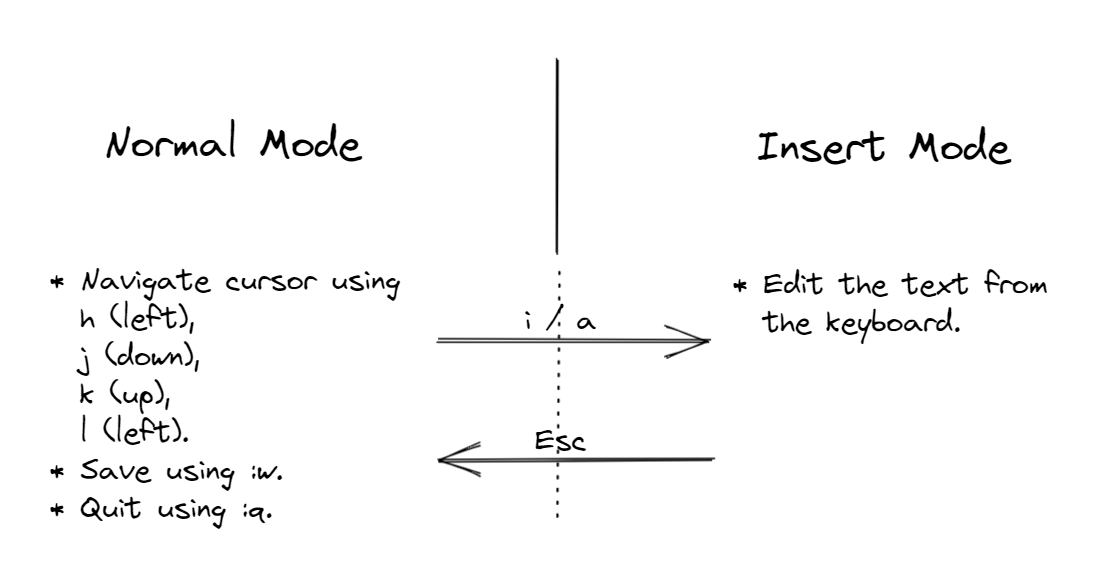
\includegraphics[width=250pt]{chapters/part-1/figures/vimbasicmodeswitching.png}
\caption{Mode switching between normal mode and insert mode, and basic functions associated with the modes.} \label{ch:tfe:fig:vimbasicmodeswitching}
\end{figure}

\begin{figure}[!htb]
\centering
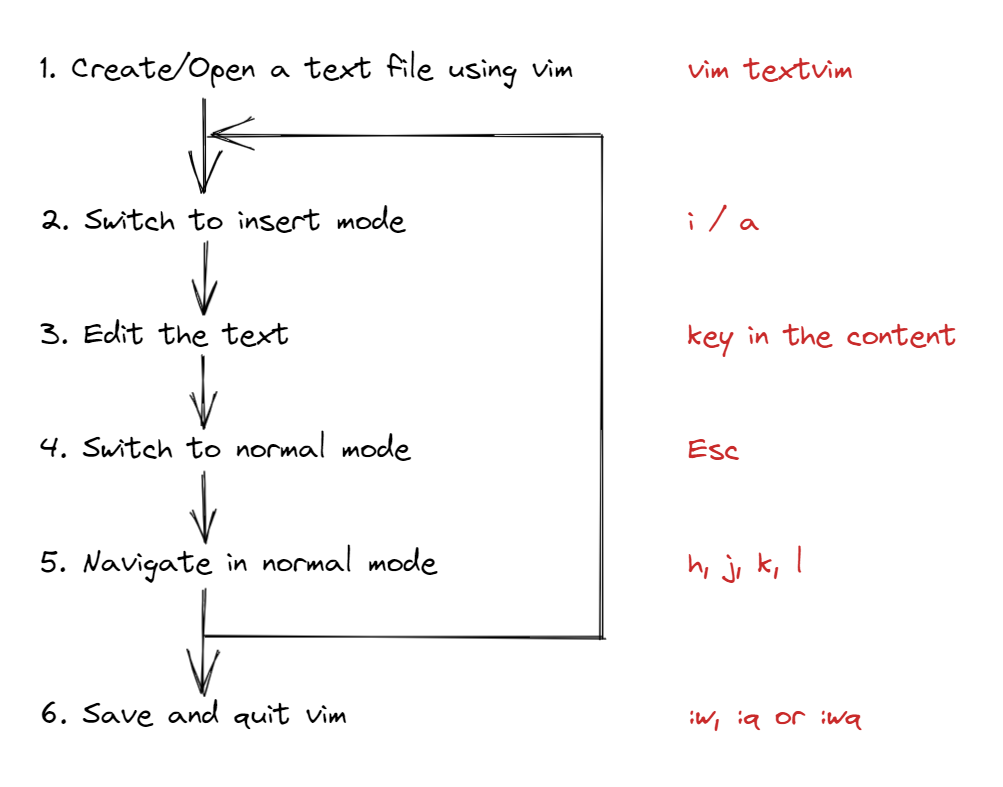
\includegraphics[width=250pt]{chapters/part-1/figures/vimbasicoperationflowchart.png}
\caption{A flowchart for simple creating, editing and saving of a text file using Vim.} \label{ch:tfe:fig:vimbasicoperationflowchart}
\end{figure}

There are other shortcuts to switch from normal mode to insert mode. Some of them are summarized in Table \ref{ch:tfe:tab:switchtoinsert}.

\begin{table}
  \centering \caption{Commonly used shortcuts to switch from normal mode to insert mode.}\label{ch:tfe:tab:switchtoinsert}
  \begin{tabularx}{\textwidth}{lX}
    \hline
    Operator & Description \\ \hline
    \verb|i| & Insert before the character at the cursor. \\ 
    \verb|I| & Insert at the beginning of the row at the cursor. \\ 
    \verb|a| & Insert after the character at the cursor. \\ 
    \verb|A| & Insert at the end of the row at the cursor. \\ 
    \verb|o| & Create a new row below the cursor and switch to insert mode. \\ 
    \verb|O| & Create a new row above the cursor and switch to insert mode. \\
    \hline
  \end{tabularx}
\end{table}

\section{Vim Profile Configuration}

With the basic operations introduced in Section \ref{ch:tfe:subsec:vimgeneralintro}, we are able to create and edit a text file as we want to, just like using any other text editor. Though at this point the advantages of using Vim over other text editors are not obvious yet, the Vim editor is at least useable.

Before introducing more advanced features of Vim, for better user experience we can now customize the user profile to suit our individual habit. Notice that the customization is completely optional and personal. This section only introduces the idea and basic methods such as re-mapping keys and creating user-defined shortcuts. Everything introduced here are merely examples and it is completely up to the user how to design and implement his own profile.

In Linux, navigate to home directory. Create the following path and file \verb|~/.vim/vimrc| or \verb|~/.vimrc|. Open the \verb|vimrc| file as a blank file using Vim. The individual user profile can be customized here.

There are many readily available \verb|vimrc| profiles shared in the community. Feel free to use them as a reference when creating a new profile.

\subsection{Mapping Shortcuts}

It is desirable to re-map some keys to speed up the text editing. For example, by mapping \verb|jj| to \verb|Esc| in insert mode, one can switch from insert mode to normal mode more quickly (notice that consequent ``jj'' is rarely used in English). Another example coud be mapping \verb|j|, \verb|k|, \verb|i| to \verb|h|, \verb|j|, \verb|k| respectively in normal and visual modes, making the navigation more intuitive. In that case, another key needs to be mapped to \verb|i| because insert command is very useful and we do not want to lose it.

The mapping of keys and keys combinations can be done as follows in \verb|vimrc|.
\begin{lstlisting}
inoremap jj <Esc>
noremap j h
noremap k j
noremap i k
noremap h i
\end{lstlisting}
where \verb|inoremap| is used to map keys (combinations) in insert mode, and \verb|noremap| in normal and visual modes.

The upper case letter \verb|S| and lower case letter \verb|s| in normal mode are originally used to delete and substitute texts, and they are rarely used due to the more powerful shortcut \verb|c| which does similar tasks. We can re-map \verb|S| to saving, and disable \verb|s|. Similarly, upper case letter \verb|Q| is mapped to quitting Vim.
\begin{lstlisting}
noremap s <nop>
map S :w<CR>
map Q :q<CR>
\end{lstlisting}
where \verb|<nop>| stands for ``no operation'' and \verb|CR| stands for the ``enter'' key on the keyboard. The keyword \verb|map| differs from \verb|noremap| in the sense that \verb|map| is for recursive mapping.

\subsection{Syntax and Color Scheme}

By default Vim displays white colored contents on a black background. Use the following command in \verb|vimrc| to enable syntax highlighting or change color schemes. Use \verb|:colorscheme| in cmdline mode in Vim to check for available color schemes.
\begin{lstlisting}
syntax on
colorscheme default
\end{lstlisting}

The following setups in \verb|vimrc| displays the row index and cursor line (a underline at cursor position) of the text, which can become handy during the programming. Furthermore, it sets auto-wrap of text when a single row is longer than the displaying screen.
\begin{lstlisting}
set number
set cursorline
set wrap
\end{lstlisting}

The following command opens a ``menu'' when using cmdline mode, making it easier to key in commands.
\begin{lstlisting}
set wildmenu
\end{lstlisting}

\subsection{Other Useful Setups}

Use \verb|scrolloff| to make sure that when scrolling in Vim, there are always margins lines in the top and bottom of the screen, so that the cursor is always close to the centre of the screen.
\begin{lstlisting}
set scrolloff=3
\end{lstlisting}

Enable spell check in Vim as follows.
\begin{lstlisting}
map sc :set spell!<CR>
\end{lstlisting}
where \verb|sc| can be used to quickly turn on and off the spell check function. In addition, when the cursor is put on the wrongly spelled word, use \verb|z=| to open a list of possible corrections.

\subsection{Plug Tools}

In the Linux community, many plug tools have been created to add useful features for Vim. As a demonstration, in this section \mync{vim-plug}, a light-size vim plugin management tool created on GitHub, is used to install selected Vim plugins. Details about vim-plug can be found at GitHub under \textit{junegunn/vim-plug}.

Following the instructions given by GitHub under \textit{junegunn/vim-plug}, to use vim-plug on Linux, the very first step is to use \verb|curl|, a command-line tool for transferring data specified with URL syntax, to download vim-plug. To install \verb|curl| if it has not been installed, use
\begin{lstlisting}
$ sudo yum install curl # red-hat-based distributions
$ sudo apt install curl # debian-based distributions
\end{lstlisting}

With \textit{cURL} installed, use the following in the shell to install vim-plug
\begin{lstlisting}
$ curl -fLo ~/.vim/autoload/plug.vim --create-dirs \
    https://raw.githubusercontent.com/junegunn/vim-plug/master/plug.vim
\end{lstlisting}
In the very beginning of \verb|vimrc|, add the following to specify the plugins to be installed. As an example, \textit{vim-airline/vim-airline} and \textit{joshdick/onedark.vim} are to be installed, the first of which adds a status line at the bottom of the Vim window, and the second adds a popular color scheme ``onedark''.
\begin{lstlisting}
call plug#begin()
Plug 'vim-airline/vim-airline'
Plug 'joshdick/onedark.vim'
call plug#end()
\end{lstlisting}
Finally, reload \verb|vimrc|, then run \verb|:PlugInstall| in cmdline mode to install the plugins. Use \verb|colorscheme onedark| instead of \verb|colorscheme default| in \verb|vimrc| to enjoy the onedark color scheme.

Notice that instead of setting up configurations permanently in \verb|vimrc|, the user can also apply a setup in cmdline mode for temporary use in an open session. A full list of \verb|vimrc| configurations used in this chapter can be found in the appendix.

\section{Basic Operations in Vim}

In normal mode, the most frequently used operation is probably \verb|u| for undo. Other commonly used operations, such as delete, cut, copy, paste, replace and search, are mostly done in normal mode through shortcut keys. For example, \verb|dd| deletes (cuts) the entire row at the cursor and \verb|p| pastes the content in the clipboard to the cursor position. For beginners, remembering shortcut keys can be difficult. Therefore, it is suggested looking for the consistent patterns of the different commands, rather than brute-force remembering all the operations.

Many Vim shortcut keys in normal mode has the following pattern: an operator command directly followed by a motion command without space in between.
\begin{lstlisting}
<operator><motion>
\end{lstlisting}
The operator command tells Vim what to do (say, copy), and the motion command tells the applicable range of the operation (say, a row, or a word, or a character). Some operator commands may work alone without motion commands.

\subsection{Cut, Change, Copy and Paste}

The following lines taken from Wikipedia under ``William Shakespeare'' is used as an example to demonstrate delete/cut, change, copy and paste functions. In the text file, each sentence takes a separate row as shown in Figure \ref{ch:tfe:fig:vimdemo1}.

\begin{shortbox}
William Shakespeare (bapt. 26 April 1564 – 23 April 1616) was an English playwright, poet and actor, widely regarded as the greatest writer in the English language and the world's greatest dramatist.

He is often called England's national poet and the ``Bard of Avon'' (or simply ``the Bard'').
\end{shortbox}

\begin{figure}[htbp]
\centering
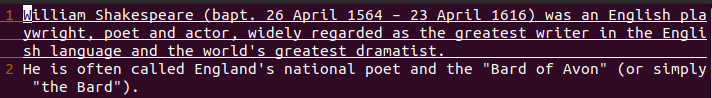
\includegraphics[width=250pt]{chapters/part-1/figures/vimdemo1.png}
\caption{A piece of text of ``William Shakespeare'', for demonstration.} \label{ch:tfe:fig:vimdemo1}
\end{figure}

Use either \verb|x| or \verb|X| to delete the character at the cursor or previous to the cursor, respectively. To delete multiple characters, one way is to press \verb|x| or \verb|X| multiple times (or hold the keys). Alternatively, it is possible for Vim to automatically repeat the procedure. For example, \verb|20x| tells Vim to perform \verb|x| for 20 times. The same applies for other operators or motions commands. For example, \verb|10l| executes \verb|l| for 10 times, moving the cursor to the right for 10 characters.

Operator \verb|d|, similar with \verb|dd|, deletes the contents of the text, but it requires a motion command and can be used more flexibly. The motion shall tell Vim the applicable range to delete/cut.

For example, \verb|dl| deletes one character to the right, i.e. deletes the character at the cursor just like \verb|x|. Likewise, \verb|dh| deletes one character to the left just like \verb|X|. Similarly, \verb|d20l| deletes 20 characters to the right, where ``20l'' as a whole plays as the motion of ``20 characters to the right''. A combination by using things like \verb|5d4l| also works and leads to the same result as $20=5\times 4$.

Command \verb|d| can be used even more flexibly. For example, by using word-related motions, \verb|d| can delete/cut by words instead of by characters. Move the cursor to the beginning of a word, (for example, ``S'' in ``Shakespeare''), use \verb|dw| to delete the word. The word motion \verb|w| is similar with \verb|l|, except that \verb|l| directs to the next character, while \verb|w| directs to the beginning of next word. Similarly, \verb|b| directs to the beginning of the current/previous word. Thus, \verb|db| can be used to delete word to the left. Examples \verb|d10b|, \verb|10db|, \verb|d20w|, \verb|5d4w| can be used to delete multiple words at a time. Motions \verb|w| and \verb|b| can also be used to navigate in the text just like \verb|l| and \verb|h|.

When in the middle of a word, \verb|dw| will delete the characters from the cursor to the beginning character of the next word. For example, if the cursor is currently at ``k'' in ``Shakespeare'', \verb|dw| will delete ``kespeare '' (notice that the space between ``Shakespeare'' and ``(bapt.'' will also be deleted). To delete from the beginning of the word instead, you can use \verb|b| first to navigate back to the beginning of the word, then apply \verb|dw|. Alternatively, use ``inner-word'' motion \verb|iw| to indicate that the whole word of the cursor shall be deleted, i.e., \verb|diw| to delete ``Shakespeare''. The space after ``Shakespeare'' will stay. To remove that space together with the word ``Shakespeare'', use \verb|daw| instead. More about motions \verb|aw| will be introduced shortly.

In addition to character-related motions \verb|h|, \verb|l| and word-related motions  \verb|b|, \verb|w|, there are similar motions for sentence \verb|(| (previous), \verb|)| (next) and paragraph \verb|{| (previous), \verb|}| (next). There are also inner-sentence motion \verb|is|, inner-paragraph motion \verb|ip|, inner-quotation motion \verb|i'|, \verb|i"|, \verb|i`| and inner-block motion \verb|i(|, \verb|i<|, \verb|i{|, and many more. For example, when the cursor is at ``A'' of ``26 April 1564'', \verb|di(| will delete everything inside ``()'', i.e. deleting ``bapt. 26 April 1564 - 23 April 1616''.

The operators and motions introduced so far are summarized in Tables \ref{ch:tfe:tab:deletecut} and \ref{ch:tfe:tab:motion}. Notice that motions \verb|aw|, \verb|as|, \verb|ap| are also given in the table. They are similar with their corresponding \verb|iw|, \verb|is|, \verb|ip| except that when deleting, the sequential blank space (for word and sentence) or blank row (for paragraph) will also be deleted.

\begin{table}[!htb]
  \centering \caption{Commonly used operators related to delete/cut, change, copy and paste.}\label{ch:tfe:tab:deletecut}
  \begin{tabularx}{\textwidth}{lX}
    \hline
    Operator & Description \\ \hline
    \verb|x| & Delete/Cut the character at cursor. \\ 
    \verb|X| & Delete/Cut the character before cursor. \\ 
    \verb|dd| & Delete/Cut the entire row. \\ 
    \verb|d| & Delete/Cut selected text according to the motion command. \\ 
    \verb|cc| & Change the entire row. \\ 
    \verb|c| & Change selected text according to the motion command. \\ 
    \verb|yy| & Copy the entire row. \\ 
    \verb|y| & Copy selected text according to the motion command. \\ 
    \verb|p| & Paste clipboard to the cursor. \\
    \hline
  \end{tabularx}
\end{table}

\begin{table}[!htb]
  \centering \caption{Commonly used motions.}\label{ch:tfe:tab:motion}
  \begin{tabularx}{\textwidth}{lX}
    \hline
    Motion & Description \\ \hline
    \verb|h|, \verb|l| & One character to the left or right. \\ 
    \verb|j|, \verb|k| & One row to the up or down. \\ 
    \verb|b| & First character of the current word, or fist character of the previous word. \\ 
    \verb|e| & Last character of the current word. \\ 
    \verb|w| & First character of the next word. \\ 
    \verb|(|, \verb|)| & One sentence to the previous or next. \\ 
    \lstinline{\{}, \lstinline{\}} & One paragraph to the previous or next. \\ 
    \verb|iw|, \verb|is|, \verb|ip| & Inner-word, inner-sentence, inner-paragraph. \\ 
    \verb|aw|, \verb|as|, \verb|ap| & A word, a sentence, a paragraph (including the end blank). \\ 
    \verb|i'|, \verb|i"|, \verb|i`| & Inner-quotation for different types of quotations. \\ 
    \verb|i(|, \verb|i<|, \verb|i[|, \lstinline{\}} & inner-block for different types of brackets. \\ 
    \verb|0| (zero) & Beginning of the row. \\ 
    \verb|$| & Ending of the row. \\ 
    \verb|gg| & Beginning of the text. \\ 
    \verb|G| & Beginning of the last row of the text. \\
    \hline
  \end{tabularx}
\end{table}

To change contents, use operator \verb|c|, which works the same way as \verb|d| but it automatically switch to insert mode after removing the content. To copy a piece of text to clipboard, use \verb|y| (stands for ``yank'') followed by its associated motion to indicate the range of text. The motions also follow Table \ref{ch:tfe:tab:motion}. To paste the text in the clipboard to the cursor, use \verb|p|. No motion is required.

In addition to Table \ref{ch:tfe:tab:motion}, another commonly used type of motion is to ``find by character''. For example, consider the following row of text. The cursor is currently at letter ``A''.
\begin{lstlisting}
ABCDEFG;HIJKLMN;OPQ;RST;UVW;XYZ
\end{lstlisting}
In normal mode, using \verb|f| followed by a character will navigate the cursor to the nearest corresponding character that appears in the text. For example, \verb|fG| will move the cursor to letter ``G''. Similarly, \verb|f;| will move the cursor to the ``;'' between ``G'' and ``H''. Key in \verb|f;| again and the cursor will move to ``;'' between ``N'' and ``O''. From here key in \verb|2f:| and the cursor will go to ``;'' between ``T'' and ``U'', as it is equivalent to executing \verb|f;| twice. If \verb|df;| is used when the cursor is at letter ``A'', ``ABCDEFG;'' will be deleted.

\subsection{Search in the Text}

In normal mode, use \verb|/<content>| to search a keyword or a phrase. The following customization in \verb|vimrc| shall give a better searching experience.

When searching in the text for a particular word or phrase (searching in the text will be will be covered in a later of the chapter), to make the searching result highlighted, add the following line to the user profile \verb|vimrc|.
\begin{lstlisting}
set hlsearch
exec "nohlsearch"
set incsearch
noremap <Space> :nohlsearch<CR>
set ignorecase
noremap = nzz
noremap - Nzz
\end{lstlisting}
where \verb|hlsearch| enables highlighting all matching results in the text, and \verb|incsearch| enables highlighting texts along with typing the keyword. Vim remembers the keyword from the previous search and may automatically highlight them in the text on a new session. This can be confusing sometimes. To tackle the issue, use command \verb|exec "nohlsearch"| (\verb|exec| in \verb|vimrc| executes a command when starting a new session) after \verb|set hlsearch| to force Vim to clear its searching memory on a new session. Finally, to quit searching, use \verb|:nohlsearch| in cmdline mode and the highlights shall be gone. For convenience, consider mapping it with a customized shortcut key as well, for example to \verb|Space|. As a bonus, set \verb|ignorecase| to ignore case-sensitive during the searching.

Keys \verb|n| and \verb|N| is used to navigate through the searching result, and \verb|zz| is used to pin cursor position in the central of the screen. They are mapped to \verb|-| and \verb|=| in \verb|vimrc|. Notice that they can also be used as motion together with delete/cut, change and copy as given in Table \ref{ch:tfe:tab:deletecut}.

With the above setup, searching for ``he'' using \verb|/he| leads to the following result given in Fig.~\ref{ch:tfe:fig:vimdemo2}.
\begin{figure}[htbp]
\centering
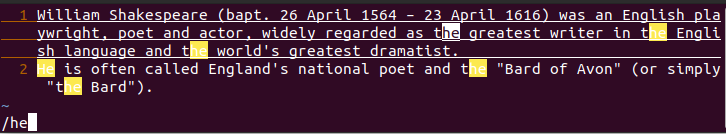
\includegraphics[width=250pt]{chapters/part-1/figures/vimdemo2.png}
\caption{Search ``he'' in the piece of text of ``William Shakespeare''.} \label{ch:tfe:fig:vimdemo2}
\end{figure}
From Fig.~\ref{ch:tfe:fig:vimdemo2}, it can be seen that all appearances of ``he'' (case-insensitive) is highlighted, and the cursor is automatically moved to its first appearance, i.e. ``he'' in ``the greatest writer''. Click \verb|Enter| to enable free move of the cursor.

\subsection{Other Tips}

Use \verb|Ctrl+o|, \verb|Ctrl+i| to ``undo'' and ``redo'' cursor positions, respectively. They only move the cursor position and don't change the actual texts.

To save as a file, use \verb|:w <new path>| in cmdline mode.

In cmdline mode, use \verb|!| to interact with the shell. For example, consider a case where a read-only file needs to be edited and saved by a sudoer who forgot to start Vim using \verb|sudo|. The common \verb|:w| will be rejected. In this case, use \verb|:w !sudo tee %| to perform the save, where \verb|tee| is a Linux command that takes standard input and writes to a file, and \verb|%| stands for the current file. In another example where an existing file's content is to be insert into the current text, navigate the cursor to the place to insert the text, and use \verb|:r !cat <filename>|.

To convert and save the current text into an \textit{html} file, use \verb|:%TOhtml|. From there, the file can be further converted into a PDF file.

\section{Visual Mode}

The use of a mouse makes selecting a block of text very intuitive. In most text editors, the selected text will be highlighted, as if the cursor expands from one character to the entire block of text. Sequentially, operations such as delete and copy can be performed on the selected text.

The three visual modes of Vim, namely ``visual'', ``visual-line'' and ``visual-block'', provide similar experience where the user can select and highlight a block of text.

Use \verb|v| to enter the visual mode, then navigate the cursor to select a block of text. This allows the user to select text between any two characters. An example is given by Fig. \ref{ch:tfe:fig:vimvm1}. Alternatively, use \verb|V| to enter the visual-line mode where multiple lines can be easily selected, and use \verb|<ctrl>+v| to enter visual-block mode to select a rectangular block of text.

\begin{figure}[htbp]
	\centering
	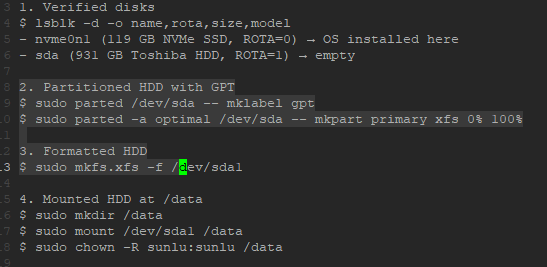
\includegraphics[width=100pt]{chapters/part-1/figures/vimvm1.png}
	\caption{An example of visual mode where a block of text is selected.} \label{ch:tfe:fig:vimvm1}
\end{figure}

In any of the above visual mode, use \verb|:normal + <operation>| to execute operation(s) form the normal mode for each line. This allows convenient editing of multiple lines of text all together. For example, use \verb|V| to select a few lines of contents, followed by \verb|:normal 0iprefix-|. This will insert \verb|prefix-| to all the lines, as if \verb|0iprefix-| is executed in normal mode to all the lines separately. Notice that if \verb|i| has been mapped by another character in normal mode, use that character instead.

Alternatively, in visual-block mode after selecting a block of content, use \verb|I| to enter insert mode and insert content in the first row of the selected block. When existing the insert mode using \verb|<Esc>|, the changes will apply to all selected rows. Similar effect can be achieved.

\section{Vim Macros}

\mync{Vim macros} allows the user to define a sequence of actions, and it is a convenient and power tool for repetitive works. Use \verb|q| in normal mode to start and end a macro recording. The syntax follows
\begin{lstlisting}
q<macro-name><operations>q
\end{lstlisting}
where \verb|<macro-name>| is a single character that labels the macro.

Consider the following example where there is a text file containing the following content
\begin{lstlisting}
apple.jpg
pear.jpg
orange.jpg
banana.jpg
peach.jpg
\end{lstlisting}
and we would like to change the content to
\begin{lstlisting}
image: 'apple.jpg'
ttl: 5
image: 'pear.jpg'
ttl: 5
image: 'orange.jpg'
ttl: 5
image: 'banana.jpg'
ttl: 5
image: 'peach.jpg'
ttl: 5
\end{lstlisting}

In this example, repetitive work is involved and it is time consuming to do it manually if there are thousands of items in the file, and it is better to record a macro to automate the procedure. Navigate the cursor to the first row of the text, and type the following sequence of characters.
\begin{lstlisting}
q<macro name>0iimage: '<Esc>A'<Enter>ttl: 5<Esc>jq
\end{lstlisting}
where \verb|<macro name>| can be any character, for example \verb|s|. The string in the middle \verb|0iimage: '<Esc>A'<Enter>ttl: 5<Esc>j| is the necessary procedure to perform the revision for one row. If everything is done correctly, the file should appear as
\begin{lstlisting}
image: 'apple.jpg'
ttl: 5
pear.jpg
orange.jpg
banana.jpg
peach.jpg
\end{lstlisting}
and the cursor should be at row \verb|pear.jpg|.

To repeat the recorded procedures, use \verb|@<macro-name>|. In this example, just key in \verb|@s| in the normal mode, and the file should appear as
\begin{lstlisting}
image: 'apple.jpg'
ttl: 5
image: 'pear.jpg'
ttl: 5
orange.jpg
banana.jpg
peach.jpg
\end{lstlisting}

Repetitively using \verb|@s| proceeds with the revision. In the case the procedure needs to be repeated for many times, use \verb|<number>@<macro-name>|, in this example \verb|3@s|, to complete the remaining task.

\section{File Explorer and Screen Splitting}

Many IDEs come with project folder navigation and screen splitting features. In these IDEs, there is often a built-in file explorer, from where the user can navigate in the file system, select a file to edit, and the IDE will split the window for the selected file. Vim has similar features that supports file explorer and screen splitting, either via built-in functions or third-party support tools.

In Vim, use \verb|:Explore|, \verb|:Sexplore| or \verb|:Vexplore| (or \verb|:Ex|, \verb|:Sex|, \verb|:Vex| for short) in cmdline mode to open a file explorer, from where the user can navigate the cursor to select a file. Vim will then open the file in a split window that allows the user to further editing the file.

There are many third-party plugin tools that enable convenient file explorer functions. For example, \textit{github.com/scrooloose/nerdtree}. More details can be found in the associated repository on \textit{GitHub}.

Use \verb|:split| and \verb|:vsplit| for horizontal and vertical screen splitting, respectively. A second split window would show up with the same text file opened. For simplicity, these commands can be mapped in \verb|vimrc| as follows.
\begin{lstlisting}
noremap sj :set nosplitright<CR>:vsplit<CR>
noremap sl :set splitright<CR>:vsplit<CR>
noremap si :set nosplitbelow<CR>:split<CR>
noremap sk :set splitbelow<CR>:split<CR>
\end{lstlisting}
where \verb|splitright| and \verb|splitbelow| is used to setup the default cursor position after splitting the screen.

In a split window, open a new file using \verb|:e <path>|. To navigate the cursor across different split windows, use \verb|Ctrl+w| followed by \verb|h|, \verb|j|, \verb|k| and \verb|l|. For simplicity, they can be mapped as follows.
\begin{lstlisting}
noremap <C-j> <C-w>h
noremap <C-l> <C-w>l
noremap <C-i> <C-w>k
noremap <C-k> <C-w>j
\end{lstlisting}
where \verb|<C->| stands for \verb|Ctrl+|.

Resize the selected split window using \verb|:res+<number>|, \verb|:res-<numer>|, \verb|:vertical resize+<number>|, \verb|:vertical resize-<number>|. For simplicity, map these commands as follows.
\begin{lstlisting}
noremap J :vertical resize-2<CR>
noremap L :vertical resize+2<CR>
noremap I :res+2<CR>
noremap K :res-2<CR>
\end{lstlisting}

\section{NeoVim}

Vim being an open-source project allows other to fork and build new projects on top of it. \mync{NeoVim} is one of those projects. Comparing with Vim whose code is almost all from Bram Moolenaar, NeoVim is more of a community-driven project with diversified contributors. 

A potential problem with project codes coming from a single contributor is that the code is often a bit more messy than if it were written and cross-checked by multiple contributors, and that has been the main criticism Vim has received. NeoVim, on the other hand, has cleaner code base. 

It seems that NeoVim is a more cutting-edge version of Vim in the sense that new features usually come sooner in NeoVim than in Vim. NeoVim also has a better and more native support for Lua language. It seems that the entire configuration file for NeoVim, i.e., the counterpart of \verb|vimrc|, can be built by Lua files. Vim is initially a single-thread application, which is fine when it is used as a text editor. However, it limits the ability of Vim calling other shell services. The user needs to wait for the shell services to end before he can start editing the document again. NeoVim, on the other hand, uses multi-thread framework, hence does not pose this issue. Later on Vim added the support to allow plug-ins to trigger multi-thread processes.

The drawback of NeoVim is that it being a younger and more collaborative project seems to be less stable than Vim.

Both Vim and NeoVim are in-development projects, and new commits are being update every day. 

\section{Other Text Editors}

Apart from Vim, many other text editors are also widely used in Linux, each with different features. For demonstration purpose, Vim and other text editors are used to open a shell script that calculates the first 10 elements of Fibonacci series.

\begin{figure}[!htb]
	\centering
	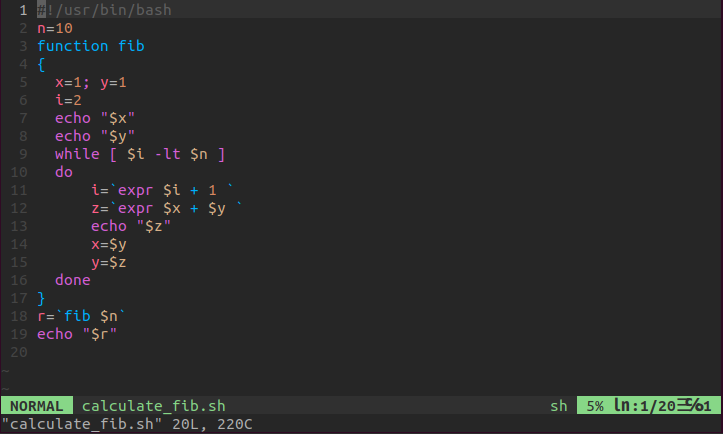
\includegraphics[width=4in]{chapters/part-1/figures/vim_fib.png}
	\caption{Vim (with user's profile customization as introduced in this chapter).}
\end{figure}

\begin{figure}[!htb]
	\centering
	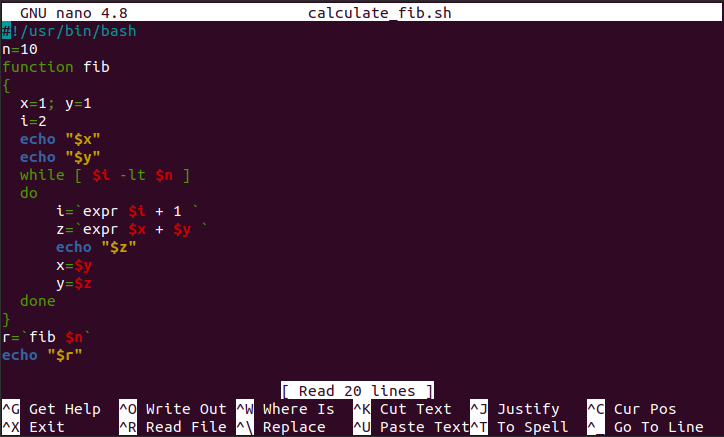
\includegraphics[width=4in]{chapters/part-1/figures/nano_fib.png}
	\caption{The nano editor.}
\end{figure}

\begin{figure}[!htb]
	\centering
	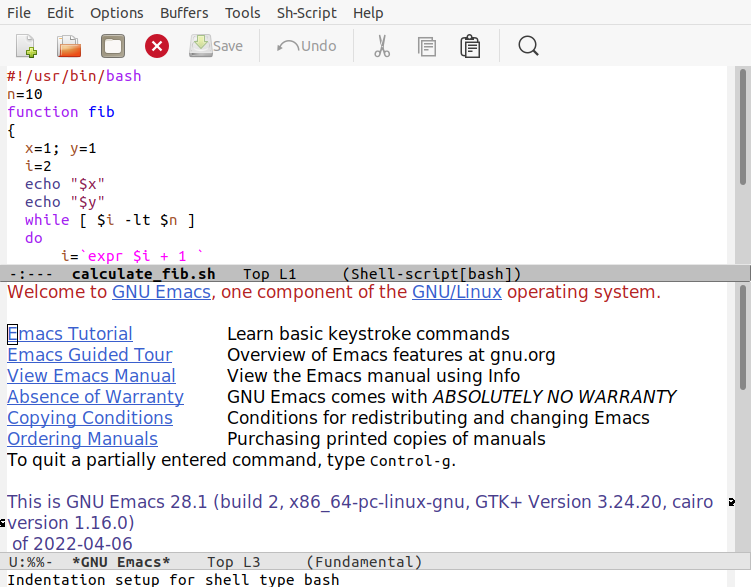
\includegraphics[width=4in]{chapters/part-1/figures/emacs_fib.png}
	\caption{The emacs editor.}
\end{figure}

\begin{figure}[!htb]
	\centering
	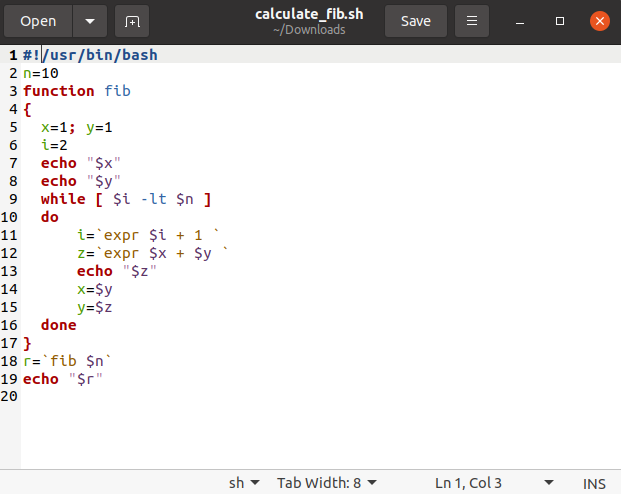
\includegraphics[width=4in]{chapters/part-1/figures/gedit_fib.png}
	\caption{The gedit editor.}
\end{figure}

\begin{figure}[!htb]
	\centering
	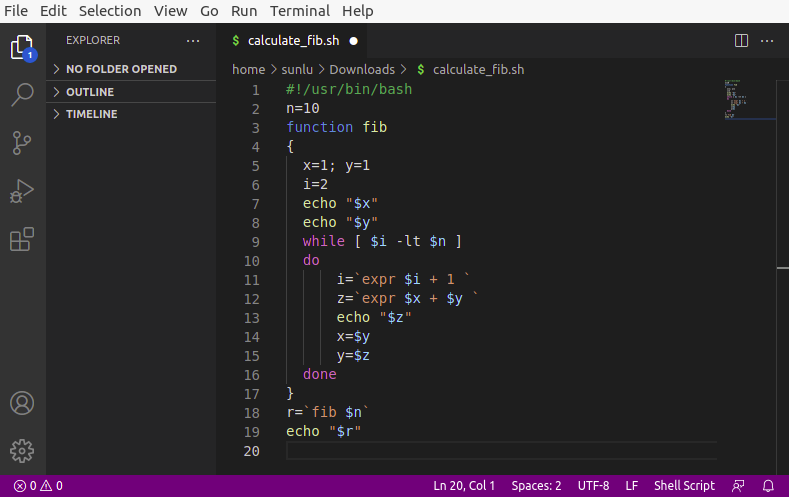
\includegraphics[width=4in]{chapters/part-1/figures/vscode_fib.png}
	\caption{Visual Studio Code.}
\end{figure}
